\documentclass[11pt,a4paper]{article}
\usepackage[T1]{fontenc}
\usepackage[utf8]{inputenc}
\usepackage{lmodern}
\usepackage[margin=2.5cm]{geometry}
\usepackage{microtype}
\usepackage{booktabs}
\usepackage{amsmath,amssymb}
\usepackage{graphicx}
\usepackage{caption}
\usepackage{enumitem}
\usepackage[authoryear,round]{natbib}
\usepackage[colorlinks=true,linkcolor=black,citecolor=black,urlcolor=blue]{hyperref}
\setlist{itemsep=2pt,topsep=4pt}
\renewcommand{\arraystretch}{1.1}
\captionsetup{font=small,labelfont=bf}

\title{\textbf{Online Ensemble Forecasting of Great Britain Day-Ahead Electricity Prices under a Strict Information Set}\\[4pt]
\large Bernstein aggregation of a diverse model pool, quantiles by QRA with adaptive conformal calibration, and a battery-dispatch evaluation}
\author{Tim-Louis Wilken}
\date{Working paper, revised 20 October 2026\\[2pt]
\small Code and outputs: \url{https://github.com/TimLouisWilken/gb-dayahead-research}}

\begin{document}
\maketitle

\begin{abstract}
\noindent
This paper forecasts the 24 hourly day-ahead prices of the Great Britain (GB) market with a pool of 13 models. All models are updated daily. They are combined per delivery hour with Bernstein Online Aggregation (BOA). The decision time is 07:30~UTC on the day before delivery. At that time the demand, wind, solar, fuel and weather inputs of the auction morning are not yet final. All inputs are checked for leakage with an automated perturbation test. Over 2024-01-01 to 2026-09-27 (about 1\,000 local days) the best combination, built from six members chosen on 2024 only, reaches MAE 8.56~EUR/MWh and rMAE 0.391 against a similar-day naive forecast; the LEAR benchmark with daily recalibration reaches 11.07. Updating the models every day is the largest single gain (random forest $-32\%$, LSTM $-21\%$ MAE against the same model trained once). For quantiles, the realised price is regressed on the 13 point forecasts and two pinball-loss boosting tail forecasts (QRA). The quantiles are then recalibrated with adaptive conformal inference. The resulting 90\,\% interval covers 89.6\,\% of hours. A linear-programme battery backtest (100~MWh / 50~MW) earns 93.1\,\% (2025) and 93.7\,\% (2026) of perfect-foresight profit. Negative results are reported as well. Seven feature sets, several combiner variants and an outage-based spike signal did not help. No claim of superiority over published methods is made. No open benchmark exists for GB, and the naive benchmark used here differs from the literature standard.
\end{abstract}

\noindent\textbf{Keywords:} electricity price forecasting, day-ahead market, Great Britain, forecast combination, online learning, quantile regression averaging, conformal prediction, battery storage.

\section{Introduction}

Day-ahead prices in Great Britain moved through three regimes in five years: the 2021--22 energy crisis, a normalisation in 2023--24, and since 2025 a market with low midday and sharp evening-ramp prices, with gas about 40\,\% higher in 2026 than in 2025. A model fitted once degrades under this drift. The question of this paper is practical. How much accuracy does a forecaster gain if every model is updated every day, and if the models are combined by an algorithm that also adapts every day?

The electricity price forecasting (EPF) literature gives a clear methodological frame (\citealp{lago2021}; \citealp{weron2014}): test over at least a year, recalibrate daily, choose hyper-parameters before the test period, report relative errors and Diebold--Mariano tests, and include a cheap strong benchmark. This paper follows that frame and adds three elements that the open benchmark does not cover. First, GB is not one of its five markets. Second, a strict information set is fixed at 07:30~UTC on day $D\!-\!1$, and every input is audited against it. Look-ahead through revised data, reanalysis weather and post-auction forecasts is the most common silent error in applied EPF. Third, the forecasts are judged by statistical scores and by the profit of a battery that trades on them.

\paragraph{Contributions.}
\begin{enumerate}
\item A leakage-audited data set and protocol for GB day-ahead prices, including seven concrete leakage patterns found in typical pipelines and in the first version of this project (Section~\ref{sec:data}).
\item A 13-member online pool (random forests, boosting, four neural architectures, LEAR, a merit-order regression and a zero-shot foundation model), combined per hour by BOA, with a documented ablation showing that six diverse members beat all thirteen (Section~\ref{sec:point}).
\item A probabilistic layer, QRA over 15 regressors followed by adaptive conformal inference, whose 50/80/90\,\% intervals are within about one percentage point of nominal (Section~\ref{sec:prob}).
\item An economic evaluation by battery dispatch and a documented list of negative results (Sections~\ref{sec:econ}, \ref{sec:negative}).
\end{enumerate}
The work was positioned against 25 papers read in full text. The positioning and its limits are in \texttt{docs/LITERATURE.md} of the repository.

\section{Data and information set}
\label{sec:data}

The target is the hourly GB day-ahead price in EUR/MWh for each local (UK) delivery day $D$. Daylight-saving days are mapped to 24 hours as in \texttt{epftoolbox}: the missing spring hour is interpolated, the doubled autumn hour is averaged. Prices come from Ember (CC-BY-4.0) up to the latest published day and from the Nord Pool N2EX result in the live system.

\paragraph{Information set.} The forecast for day $D$ is issued at 07:30~UTC on $D\!-\!1$, before the GB gate closures (EPEX 09:20, N2EX 09:50 UK time). Table~\ref{tab:inputs} lists the inputs and the availability rule that was enforced for each.

\begin{table}[ht]
\centering\small
\begin{tabular}{p{4.6cm}p{9.6cm}}
\toprule
Input & Availability rule used\\
\midrule
Prices & only complete local days $\le D\!-\!1$ (lags 1, 2, 7 and daily statistics)\\
Wind forecast, transmission (WINDFOR) & latest issue $\le$ 07:30 UTC on $D\!-\!1$\\
Embedded wind and solar (NESO) & latest issue $\le$ 07:30 UTC on $D\!-\!1$\\
Temperature forecast (Birmingham) & forecast made 48 h before each valid hour (Open-Meteo previous runs)\\
National demand forecast (NDF) & latest issue $\le$ 09:00 UK time on $D\!-\!1$ (the full-day issue appears at 08:45)\\
Demand outturn & days $\le D\!-\!2$\\
Gas (SAP) & gas day $D\!-\!3$; UK ETS (UKA) futures settlement of $D\!-\!2$\\
\bottomrule
\end{tabular}
\caption{Inputs and availability rules.}
\label{tab:inputs}
\end{table}

The demand forecast matters. It is three times more accurate than the previous proxy, the outturn one week earlier (MAE 665 vs.\ 2\,031~MW against outturn). It lowers the MAE of the 4-member hybrid by 4.9\,\%.

\paragraph{Leakage audit.} An audit of common pipeline designs and of the first version of this project found and removed the following:
(i)~a rolling price mean containing hours of the forecast day (\texttt{closed='left'} on an hourly index);
(ii)~gas and carbon lagged by only one day and a demand shift of 24 hours;
(iii)~weather taken from reanalysis (actual weather) and, in the first version, a previous-day forecast issued after the auction;
(iv)~"day-ahead" wind and solar forecasts that are published at 16:45~UTC on $D\!-\!1$, after the auction;
(v)~UTC days instead of local days, so that in summer an input hour belonged to the auction being forecast;
(vi)~gap filling with later values;
(vii)~revised wind outturn published after the cutoff (114 of 97\,000 half-hours), found by the issue-time check itself.
Two further data errors were fixed: gas SAP is in p/kWh, and a file labelled "UK ETS" was the EU ETS price. The script \texttt{src/test\_leakage.py} scrambles every value that was unknown at 07:30~UTC (prices from $D$, demand from $D\!-\!1$, gas from $D\!-\!2$, and so on), including both daylight-saving switch days, and asserts that the model inputs for $D$ are bit-identical. A positive control scrambles the permitted inputs and must change the result; a third check verifies that no forecast issue time exceeds the cutoff. 

\section{Models and combination}
\label{sec:point}

\subsection{Protocol}
Models are first fitted on 2021-07-07 to 2023-06-30. From then on each day, every member forecasts day $D$ from information before $D\!-\!1$ 07:30 and then learns the realised prices. The second half of 2023 is a burn-in used to warm up combiners and to choose hyper-parameters. All results use \textbf{2024-01-01 to 2026-09-27}, which no design choice has seen except where stated (selection on 2024 with a 2025--26 holdout).

\subsection{Members}
Table~\ref{tab:members} lists the pool. Prices are asinh-transformed for stability \citep{uniejewski2018}; neural members use reversible instance normalisation so that the network learns shapes rather than regime levels (burn-in MAE of the LSTM 16.9 $\to$ 13.5).

\begin{table}[ht]
\centering\small
\begin{tabular}{p{2.5cm}p{6.2cm}p{5.2cm}}
\toprule
Member & Model & Update scheme\\
\midrule
\texttt{lstm}, \texttt{tcn}, \texttt{transformer}, \texttt{dnn} & seq2seq LSTM, temporal CNN, encoder--decoder Transformer, MLP; 7-day history to 24 hours & daily fine-tuning with experience replay; cold refit every 91 days\\
\texttt{ddnn} & LSTM with Johnson-SU output (distribution) & as above\\
\texttt{rf\_long}, \texttt{rf\_short} & random forest, 3-year window with recency weights; 84-day window & weekly; daily\\
\texttt{lstm\_rf} & LSTM plus random forest fitted to the LSTM's out-of-sample errors & weekly\\
\texttt{gbm} & histogram gradient boosting, \emph{absolute} loss, extra fuel and wind-error features & weekly, time-ordered early stopping\\
\texttt{lear}, \texttt{lear4} & LEAR with asinh transform, 182/728-day windows (averaged), and four windows & daily recalibration\\
\texttt{merit} & merit-order regression: residual-load spline $\times$ CCGT fuel cost & daily, 182-day window\\
\texttt{chronos} & Chronos-Bolt small, zero-shot, 28-day context & none\\
\bottomrule
\end{tabular}
\caption{The 13 members. Two further quantile-loss boosting models (\texttt{gbm\_q10}, \texttt{gbm\_q90}) enter only the probabilistic stage.}
\label{tab:members}
\end{table}

One design finding is that the absolute loss is essential for boosting. With squared loss, MAE on the burn-in is 18.3 instead of 13.7, because the model chases the 2022 spikes.

\subsection{Combination by BOA}
For each delivery hour $h$ and day $t$, BOA \citep{wintenberger2017} keeps weights $w_{t,k}$ on the $K$ experts. It updates them by a second-order exponential-weights rule. The cumulative loss then approaches that of the best expert, and of the best convex combination, at a rate $O(\log K / t)$ up to a $\log\log t$ term. The loss is absolute error. Weights are updated only after the day's prices are known. Forgetting was also tested, following \citet{berrisch2024}. A grid search on 2024, confirmed on the 2025--26 holdout (Diebold--Mariano $p=0.001$), selected \emph{no} forgetting (rate 1.0). This differs from their finding for German data. For serving, the weights of hour $h$ are averaged with those of $h\pm1$ (selected on 2024, confirmed on the holdout, $p<0.001$, $-0.03$~MAE). The update itself stays per hour. No precedent for this serving-time smoothing was found in the literature reviewed.

\section{Point-forecast results}

Table~\ref{tab:point} reports the evaluation window; rMAE is the MAE relative to a similar-day naive forecast (day $D\!-\!1$ for Tuesday to Friday, $D\!-\!7$ otherwise). The standard in \citet{lago2021} is $p(d\!-\!7)$. The two differ, so numbers should not be compared across papers.

\begin{table}[ht]
\centering\small
\begin{tabular}{lrrrr}
\toprule
Model & MAE & RMSE & rMAE & sMAPE\,\%\\
\midrule
Naive (similar day) & 21.90 & 37.22 & 1.000 & 32.2\\
RF, trained once & 17.12 & 26.94 & 0.782 & 24.0\\
LSTM, trained once & 13.50 & 22.03 & 0.617 & 20.9\\
Chronos-Bolt (zero-shot) & 14.44 & 25.89 & 0.660 & 21.3\\
Merit-order regression & 12.24 & 19.97 & 0.559 & 19.4\\
RF long window, online & 11.58 & 19.08 & 0.529 & 18.7\\
\textbf{LEAR, daily recalibration} & 11.07 & 20.11 & 0.506 & 17.5\\
Gradient boosting, online & 10.79 & 18.92 & 0.493 & 17.5\\
LSTM, online & 10.69 & 18.16 & 0.488 & 17.6\\
LSTM + RF error correction & 10.37 & 17.33 & 0.474 & 17.1\\
Transformer, online (best single) & 9.78 & 17.88 & 0.446 & 16.6\\
Equal weights, all 13 & 9.15 & 17.29 & 0.418 & 15.4\\
BOA, 4 core members & 9.63 & 16.18 & 0.440 & 16.2\\
BOA, all 13 & 8.73 & 16.40 & 0.399 & 14.9\\
\textbf{BOA, selected 6} & \textbf{8.56} & \textbf{15.72} & \textbf{0.391} & \textbf{14.7}\\
\bottomrule
\end{tabular}
\caption{Out-of-sample accuracy, 2024-01-01 to 2026-09-27, EUR/MWh. Further members are in \texttt{outputs/metrics.csv}.}
\label{tab:point}
\end{table}

\begin{table}[ht]
\centering\small
\begin{tabular}{lrrr}
\toprule
MAE & 2024 & 2025 & 2026 (to Sep)\\
\midrule
Naive & 19.14 & 22.20 & 25.23\\
LEAR & 9.87 & 10.42 & 13.56\\
Transformer, online & 9.13 & 9.52 & 10.99\\
BOA, all 13 & 7.95 & 8.63 & 9.92\\
BOA, selected 6 & 7.83 & 8.32 & 9.88\\
\bottomrule
\end{tabular}
\caption{MAE by calendar year. The absolute rise in 2026 is a market effect; rMAE stays between 0.38 and 0.41.}
\label{tab:year}
\end{table}

\paragraph{Findings.}
\begin{enumerate}
\item \textbf{Continual learning is the largest gain.} Online vs.\ static: random forest 11.58 vs.\ 17.12 ($-32\%$), LSTM 10.69 vs.\ 13.50 ($-21\%$), both $p<0.001$. Static models degrade year by year; online models do not.
\item \textbf{The ensemble beats LEAR in every year}, by $-23\%$ in MAE over the whole period (8.56 vs.\ 11.07, $p<0.001$), and beats every single member, including the best one, the Transformer (9.78).
\item \textbf{Adaptive weighting pays once the pool is heterogeneous.} For the four similar core members BOA and equal weights are close (9.63 vs.\ 9.79). With weak members in the pool (Chronos 14.4, merit 12.2) BOA beats equal weights clearly (8.73 vs.\ 9.15).
\item \textbf{Six diverse members beat all 13.} Greedy backward elimination on 2024 only keeps one member per family (\texttt{lstm\_rf, gbm, transformer, lear, merit, chronos}); on the untouched 2025--26 holdout it beats the 13-member pool (9.01 vs.\ 9.18, $p=0.002$). These figures are before the serving-time weight smoothing; over the full period the two are 8.59 vs.\ 8.74 before smoothing and 8.56 vs.\ 8.73 after it. Redundant siblings dilute the weight of their better twin. The regret bound of BOA protects against bad experts, not against correlated ones. The individually weak merit and Chronos members stay because their errors are the least correlated with the rest. This agrees with the recommendation of small ensembles in \citet{lago2021}.
\item \textbf{Error correction helps.} The random forest fitted to LSTM errors improves the LSTM (10.37 vs.\ 10.69, $p=0.006$), mostly in RMSE, i.e.\ at spikes.
\end{enumerate}

\begin{figure}[ht]
\centering
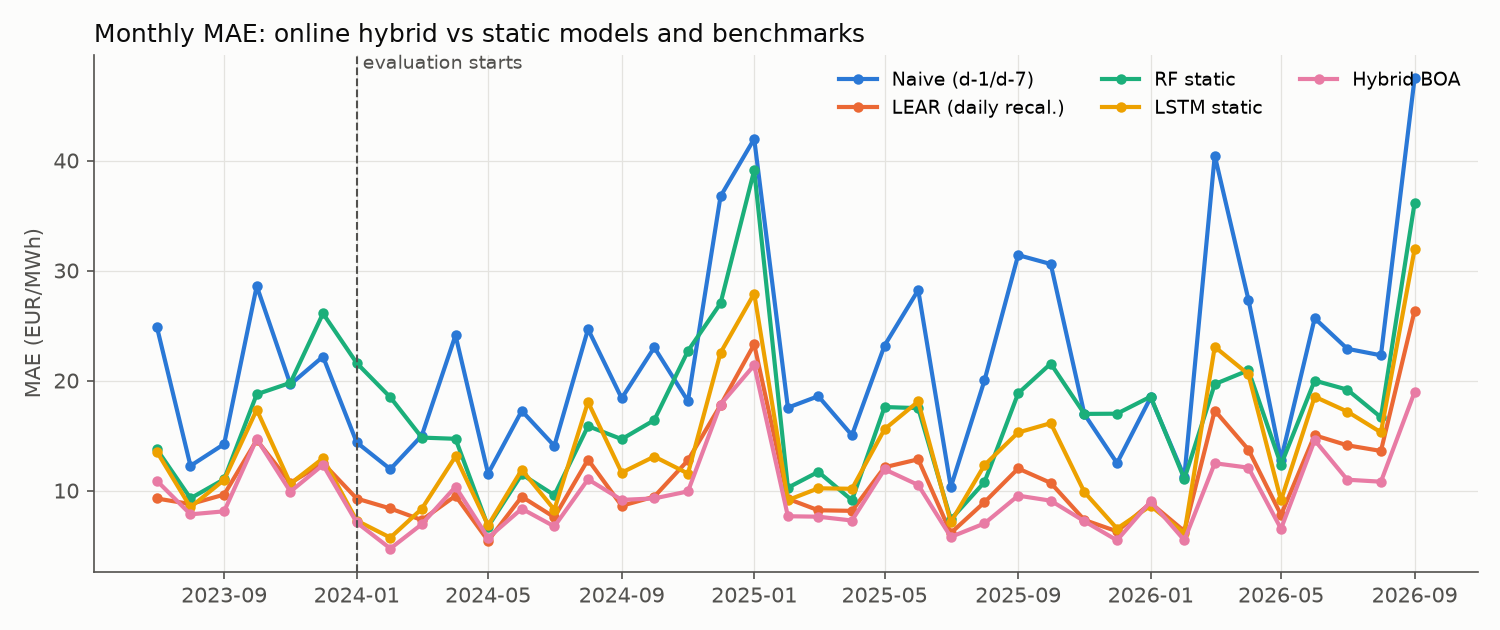
\includegraphics[width=0.9\textwidth]{../../outputs/figures/monthly_mae.png}
\caption{Monthly MAE of selected models (\texttt{outputs/figures/monthly\_mae.png}).}
\end{figure}

\section{Probabilistic forecasts}
\label{sec:prob}

\subsection{Method}
For each hour and each of 19 quantile levels ($5\%,\dots,95\%$), QRA \citep{nowotarski2015} regresses the realised price on the member forecasts over the last 182 days. The regressors are the 13 point forecasts plus the two pinball-loss boosting forecasts (QRA-15), which carry tail information that mean forecasts lack. Raw QRA is overconfident, as the literature reports \citep{kath2021}. Each quantile is therefore shifted by the matching quantile of its own past out-of-sample residuals (conformalised quantile regression). The residual level is adapted after every day from the realised hit rate (adaptive conformal inference, \citealp{gibbs2021,zaffran2022}). The step size $\gamma=0.005$ is taken from the literature range and not tuned. No published use of this two-stage combination of QRA and ACI was found.

\subsection{Results}
Table~\ref{tab:prob} reports the average pinball loss over the 19 quantiles (a proper score, about CRPS/2) and empirical coverage of central intervals.

\begin{table}[ht]
\centering\small
\begin{tabular}{lrrrrr}
\toprule
Method & Pinball & 50\,\% & 80\,\% & 90\,\% & 90\,\% width\\
\midrule
Historical simulation (BOA, core) & 3.87 & 49.2 & 78.6 & 88.3 & 41.4\\
QRA, 5 members (raw) & 3.67 & 45.6 & 74.4 & 84.6 & 36.8\\
QRA, 13 members (raw) & 3.60 & 44.2 & 72.6 & 82.7 & 35.1\\
QRA-15 (raw) & 3.58 & 44.1 & 72.3 & 82.9 & 34.5\\
QRA-13 + adaptive conformal & 3.62 & 49.1 & 79.3 & 89.6 & 45.9\\
\textbf{QRA-15 + adaptive conformal} & \textbf{3.59} & \textbf{49.4} & \textbf{79.5} & \textbf{89.6} & 43.4\\
Distributional LSTM (own output) & 3.96 & 39.3 & 67.3 & 79.3 & 34.5\\
Chronos-Bolt (own output) & 5.61 & 52.9 & 81.4 & 81.4 & 44.3\\
\bottomrule
\end{tabular}
\caption{Quantile forecasts, 2024-01-01 to 2026-09-27, daily recalibration. Coverage in percent of hours.}
\label{tab:prob}
\end{table}

Raw QRA covers only 83--85\,\% at the nominal 90\,\%. The conformal step repairs this at almost no cost in pinball loss (3.58 $\to$ 3.59). Thirteen members improve on five ($p=0.009$), and the two tail forecasts improve on the thirteen ($p=0.016$), mostly in spike hours (spike-hour pinball $-3\%$ on the selection year, confirmed on the holdout, $p=0.038$). The distributions of the neural net alone are too narrow (79\,\% at nominal 90\,\%) but useful as QRA regressors, in line with \citet{marcjasz2023}. Without LEAR in the pool, QRA gives no gain over historical simulation ($p=0.40$). The Kupiec test rejects almost every row, because about 24\,000 autocorrelated hourly hits give it extreme power. Coverage levels are therefore read directly. Per-hour Christoffersen tests are not yet reported.

\begin{figure}[ht]
\centering
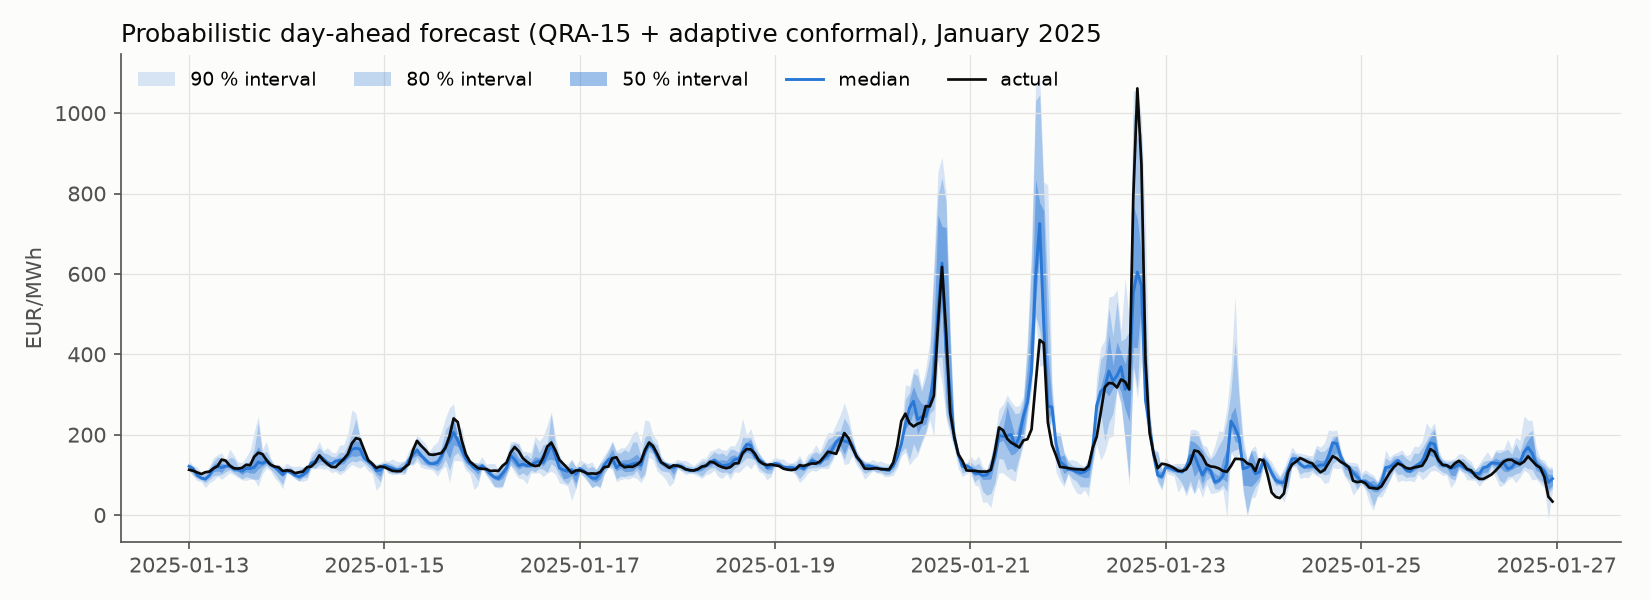
\includegraphics[width=0.48\textwidth]{../../outputs/figures/prob_fan_chart.png}\hfill
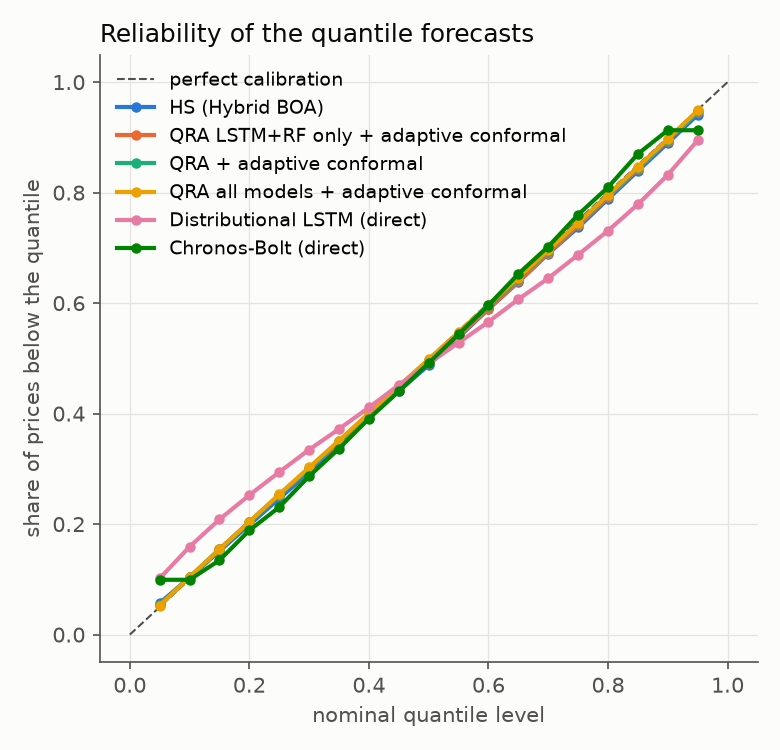
\includegraphics[width=0.48\textwidth]{../../outputs/figures/prob_reliability.png}
\caption{Fan chart of the 19 quantiles for an example period (left) and reliability diagram (right). Price data: Ember (CC-BY-4.0).}
\end{figure}

\section{Economic value: battery dispatch}
\label{sec:econ}

Accuracy measured by MAE is only loosely tied to trading value \citep{maciejowska2026}. A battery of 100~MWh / 50~MW with 85\,\% round-trip efficiency is therefore backtested. On the morning of $D\!-\!1$ a linear programme maximises profit on the \emph{forecast} of day $D$ under state-of-charge limits and a daily cycle ($SoC_{24}=0$). The schedule is committed as price-taking volume and settled at the \emph{actual} clearing prices. Profit is gross arbitrage revenue without grid charges or degradation.

\begin{table}[ht]
\centering\small
\begin{tabular}{lrrrr}
\toprule
 & \multicolumn{2}{c}{2025 (357 days)} & \multicolumn{2}{c}{2026 to Sep (270 days)}\\
Strategy & EUR/kW/yr & \% of PF & EUR/kW/yr & \% of PF\\
\midrule
Perfect foresight & 49.6 & 100.0 & 50.4 & 100.0\\
BOA, all 13 & 46.2 & 93.1 & 47.2 & 93.7\\
BOA, selected 6 & 45.7 & 92.1 & 47.2 & 93.6\\
LEAR & 44.6 & 89.9 & 45.6 & 90.4\\
Persistence (profile of $D\!-\!1$) & 37.0 & 74.5 & 38.6 & 76.5\\
\bottomrule
\end{tabular}
\caption{Battery arbitrage profit as a share of perfect foresight (PF).}
\label{tab:bess}
\end{table}

The ensemble recovers more than 92\,\% of perfect-foresight profit, LEAR about 90\,\%, and a naive profile 75\,\%. The 13-member BOA is slightly \emph{better} for dispatch than the six-member one, although its MAE is worse. Ranking skill matters for arbitrage (hit rate for the four most expensive hours 82.8 vs.\ 82.5\,\%), level skill for MAE. In the same way the LSTM+RF member has better MAE than the plain LSTM but earns less (90.3 vs.\ 91.6\,\% of PF). This reproduces, on GB data, the finding of \citet{maciejowska2026} that curve shape matters more than MAE. Absolute shares cannot be compared with other papers because strategy and market differ.

\section{Negative results}
\label{sec:negative}

Rejected ideas are reported because each was tested under the same protocol (burn-in first, then a full online A/B on the evaluation window).

\begin{itemize}
\item \textbf{Neighbour-market prices} (FR, NL, BE, NO, IE, DK, DE) and rolling price statistics: every member slightly worse (hybrid 9.79 $\to$ 9.89).
\item \textbf{Fuel and wind-error features} (TTF, EUA, wind forecast error): better for boosting only (10.85 $\to$ 10.79, every year), worse for the LSTM; adopted for \texttt{gbm} alone.
\item \textbf{Four-city temperature} and heating-degree features: better on burn-in, worse in the online A/B ($p=0.92$).
\item \textbf{Operating-margin surplus (NESO OC2):} neutral in 2024, $p=0.31$ in the full A/B.
\item \textbf{Outage information (REMIT):} falsified at the data level. Planned outages are \emph{anti}-correlated with spikes (20.4~GW unavailable on spike hours vs.\ 21.8 on normal hours in 2024), because maintenance is scheduled into calm periods. The short-notice variant has no discriminating power.
\item \textbf{Combiner variants:} forgetting, seasonal BOA states, spike-probability gating, a random-forest correction of the combination (9.13 vs.\ 8.59), a conditional median shift, QRA-$q_{50}$ as the point forecast (9.08 vs.\ 8.59), asinh-space BOA, winsorised members, a weighted median. The baseline of 8.59 is the six-member BOA before the serving-time weight smoothing, which lowers it to 8.56.
\item \textbf{Six-seed Transformer ensemble:} better alone (9.61 vs.\ 9.78) but neutral inside the combination on the selection year, so not adopted.
\end{itemize}

The QRA-$q_{50}$ result is consistent with the literature on forecast combination. The median of QRA is an unconstrained least-absolute-deviation combination, and unconstrained weights are reported to perform poorly for point forecasts \citep{weron2014,nowotarski2016}. QRA is the right tool for quantiles, not for the point forecast.

\section{Limitations}

\begin{itemize}
\item \textbf{No common GB benchmark.} The \texttt{epftoolbox} DNN was not run on this data set. The LEAR used here is a re-implementation. A rank claim against published methods is therefore not possible. rMAE against $p(d\!-\!7)$ was not computed either.
\item \textbf{Selection effects.} The 6-member subset and several hyper-parameters were selected on 2024 and confirmed on 2025--26. The holdout was reused for more than one decision. The $p$-values from Diebold--Mariano tests on 24 hourly series per day are conditional on this.
\item \textbf{Data revisions.} Demand outturn and some gas and weather series are final values. A small look-ahead effect remains. It is mitigated by lags of at least two days. Re-running the data download revises history. A/B baselines must therefore be recomputed on the same data state.
\item \textbf{Probabilistic evaluation.} Per-hour Christoffersen and multivariate Giacomini--White tests are open. The vertical average of QRA, conformal and isotonic regression \citep{lipiecki2024} was not tested on QRA-15. The step size $\gamma=0.005$ is below the values studied by \citet{zaffran2022}.
\item \textbf{Economic evaluation} uses gross arbitrage on the day-ahead market only, one battery size, no degradation and no imbalance or intraday trading.
\item \textbf{Regime.} 2026 contains an unusual spike regime (28.5\,\% of September hours above the trailing 97.5\,\% quantile); results in other regimes may differ.
\item \textbf{Sources.} Not all literature could be read in full (see Section~1 of \texttt{docs/LITERATURE.md}); one downloaded paper on calibration windows remains unread.
\end{itemize}

\section{Conclusion}

On GB day-ahead prices, with a strict 07:30~UTC information set, daily updating of every model and per-hour BOA over a diverse pool cut the MAE of the LEAR benchmark by 23\,\% (8.56 vs.\ 11.07~EUR/MWh) over 2.75 years. The combination was the best forecast in every year and in the battery backtest. Diversity mattered more than size. Six models from different families beat thirteen. QRA over point forecasts, with two tail forecasts and adaptive conformal calibration, yields intervals with near-nominal coverage. The same pipeline runs daily in production (a GitHub Actions workflow) and publishes its forecasts and monthly accuracy statistics on a public website. Next steps are the open comparisons named under the limitations. These are a common GB benchmark with the $p(d\!-\!7)$ naive, per-hour calibration tests, and the vertical average of distributional post-processors.

\section*{Reproducibility and data statement}
Code, predictions of all members, metrics, Diebold--Mariano tables and figures are in the public repository. Raw third-party price data are not redistributed (licences of Nord Pool and others); Ember data (CC-BY-4.0) can be downloaded with \texttt{src/update\_data.py}. Full-text PDFs of cited papers are not committed. The script \texttt{literature/download.sh} re-downloads them. Prices: Ember, \emph{European wholesale electricity price data}, CC-BY-4.0.

\section*{Acknowledgements}
The literature review and parts of the implementation were carried out with the help of the AI assistant Claude (Anthropic). All numbers in this paper are taken from the repository outputs.

\begin{thebibliography}{99}\small
\bibitem[Berrisch and Ziel(2024)]{berrisch2024} Berrisch, J., Ziel, F. (2024/25). Multivariate probabilistic CRPS learning with an application to day-ahead electricity prices. \emph{International Journal of Forecasting}. arXiv:2303.10019.
\bibitem[Gibbs and Cand\`es(2021)]{gibbs2021} Gibbs, I., Cand\`es, E. (2021). Adaptive conformal inference under distribution shift. \emph{NeurIPS}. (Not read in full.)
\bibitem[Kath and Ziel(2021)]{kath2021} Kath, C., Ziel, F. (2021). Conformal prediction interval estimations with an application to day-ahead and intraday power markets. \emph{International Journal of Forecasting} 37, 777--799.
\bibitem[Lago et al.(2021)]{lago2021} Lago, J., Marcjasz, G., De Schutter, B., Weron, R. (2021). Forecasting day-ahead electricity prices: a review of state-of-the-art algorithms, best practices and an open-access benchmark. \emph{Applied Energy} 293, 116983.
\bibitem[Lipiecki et al.(2024)]{lipiecki2024} Lipiecki, A., Uniejewski, B., Weron, R. (2024). Postprocessing of point predictions for probabilistic forecasting of day-ahead electricity prices: the benefits of using isotonic distributional regression. arXiv:2404.02270.
\bibitem[Maciejowska et al.(2026)]{maciejowska2026} Maciejowska, K., Lipiecki, A., Uniejewski, B. (2026). Statistical and economic evaluation of forecasts in electricity markets: beyond RMSE and MAE. arXiv:2511.13616.
\bibitem[Marcjasz et al.(2023)]{marcjasz2023} Marcjasz, G., Narajewski, M., Weron, R., Ziel, F. (2023). Distributional neural networks for electricity price forecasting. \emph{Energy Economics} 125, 106843.
\bibitem[Nowotarski and Weron(2015)]{nowotarski2015} Nowotarski, J., Weron, R. (2015). Computing electricity spot price prediction intervals using quantile regression and forecast averaging. \emph{Computational Statistics} 30(3), 791--803.
\bibitem[Nowotarski and Weron(2016)]{nowotarski2016} Nowotarski, J., Weron, R. (2016). To combine or not to combine? Recent trends in electricity price forecasting. HSC Research Report HSC/16/01.
\bibitem[Uniejewski et al.(2018)]{uniejewski2018} Uniejewski, B., Weron, R., Ziel, F. (2018). Variance stabilizing transformations for electricity spot price forecasting. \emph{IEEE Transactions on Power Systems} 33(2), 2219--2229. (Not read in full.)
\bibitem[Weron(2014)]{weron2014} Weron, R. (2014). Electricity price forecasting: a review of the state-of-the-art with a look into the future. \emph{International Journal of Forecasting} 30(4), 1030--1081.
\bibitem[Wintenberger(2017)]{wintenberger2017} Wintenberger, O. (2017). Optimal learning with Bernstein Online Aggregation. \emph{Machine Learning} 106, 119--141.
\bibitem[Zaffran et al.(2022)]{zaffran2022} Zaffran, M., Dieuleveut, A., F\'eron, O., Goude, Y., Josse, J. (2022). Adaptive conformal predictions for time series. \emph{ICML}.
\end{thebibliography}

\end{document}
